\begin{flushleft}
\doublespacing
Til dette projekt har vi valgt at designe vores program efter GRASP principper. Herved har vi stilet efter, at vores spil har lav kobling, høj samhørighed, polymorphism, creators og information experts. Dette med henblik på, at det skal være nemt at genbruge kode til fremtidige versioner eller lignende projekter. Men det gik op for os cirka lidt over halvvejs i projektet, at vi i praksis har relativt høj kobling via dependencies. Dette gør det ikke umuligt at genbruge kode, men der skal være øje for dependencies af metoder i forskellige klasser. I en fremtidig version af spillet ville vi sørge for, at der ikke var disse koblinger med dependencies, men der var desværre ikke nok tid til at rette op på det i dette projekt, da det gik op for os ret sent i processen. Til gengæld er der, hvis der ses bort fra dependencies, et generelt lavt niveau af kobling og høj samhørighed for klasserne i programmet.\\

\subsection{Sekvensdiagrammer}
Nedenfor har vi designet to sekvensdiagrammer, der viser en oversigt af objektkald for UC01: Roll dice og en enkelt polymorphic case af landOnField metoden (se Figure \ref{RollDice} og \ref{landOnField}).

\begin{figure}[H]
    \centering
    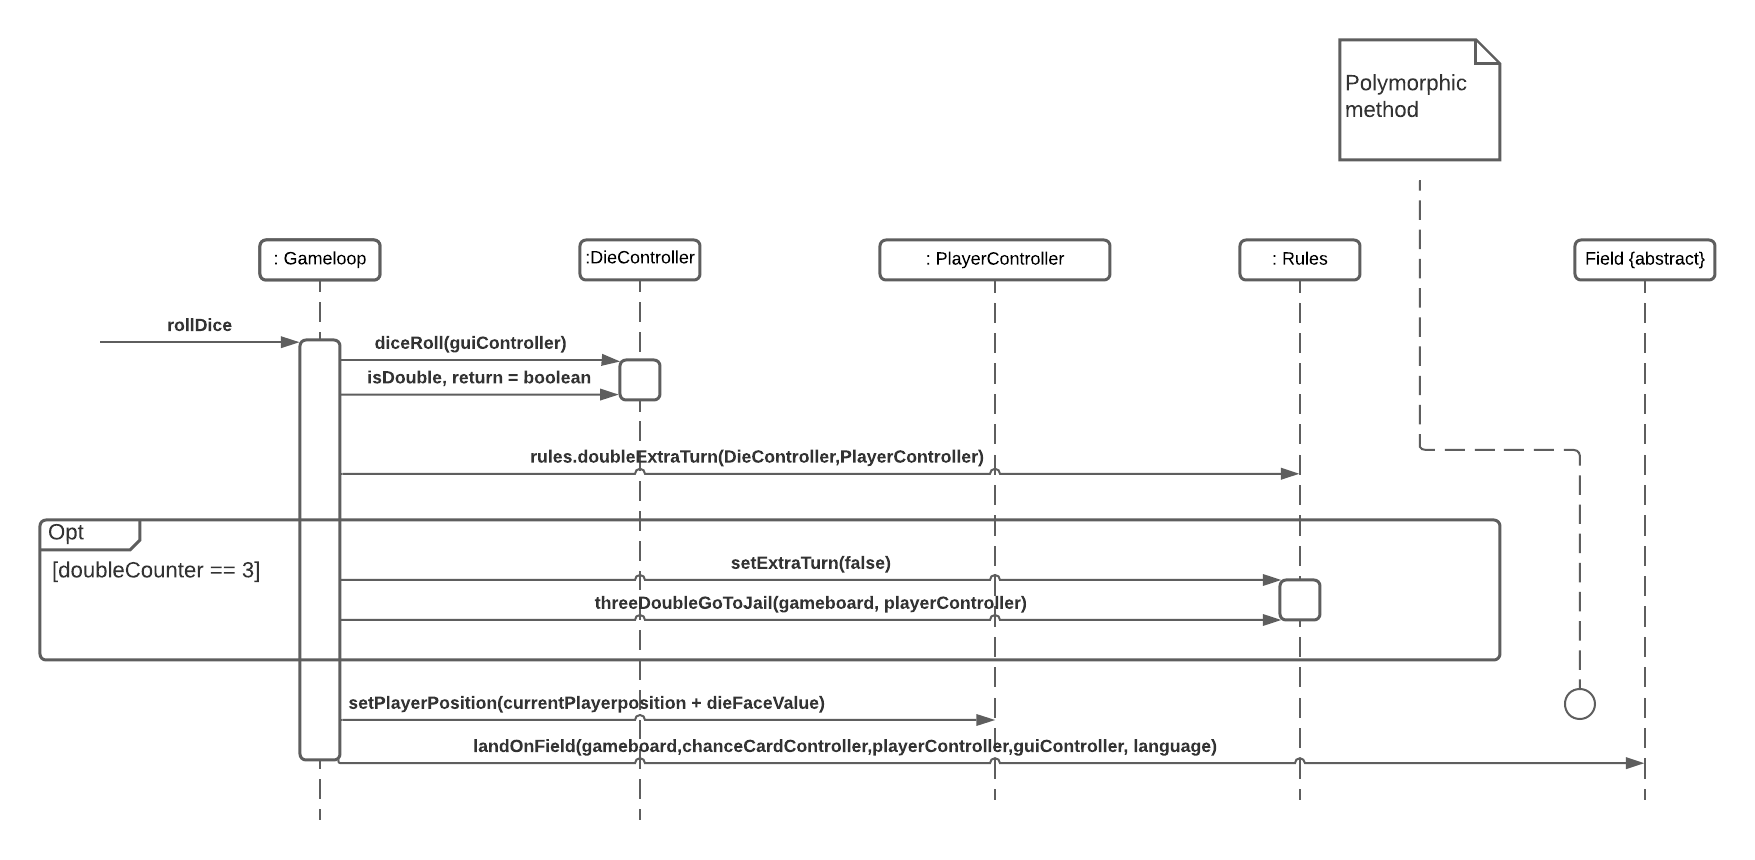
\includegraphics[width=16cm, height=10cm]{Report/figures/rollDice_sekvens.png}
    \caption{Sekvensdiagram over roll dice use-case.}
    \label{RollDice}
\end{figure}
\begin{figure}[H]
    \centering
    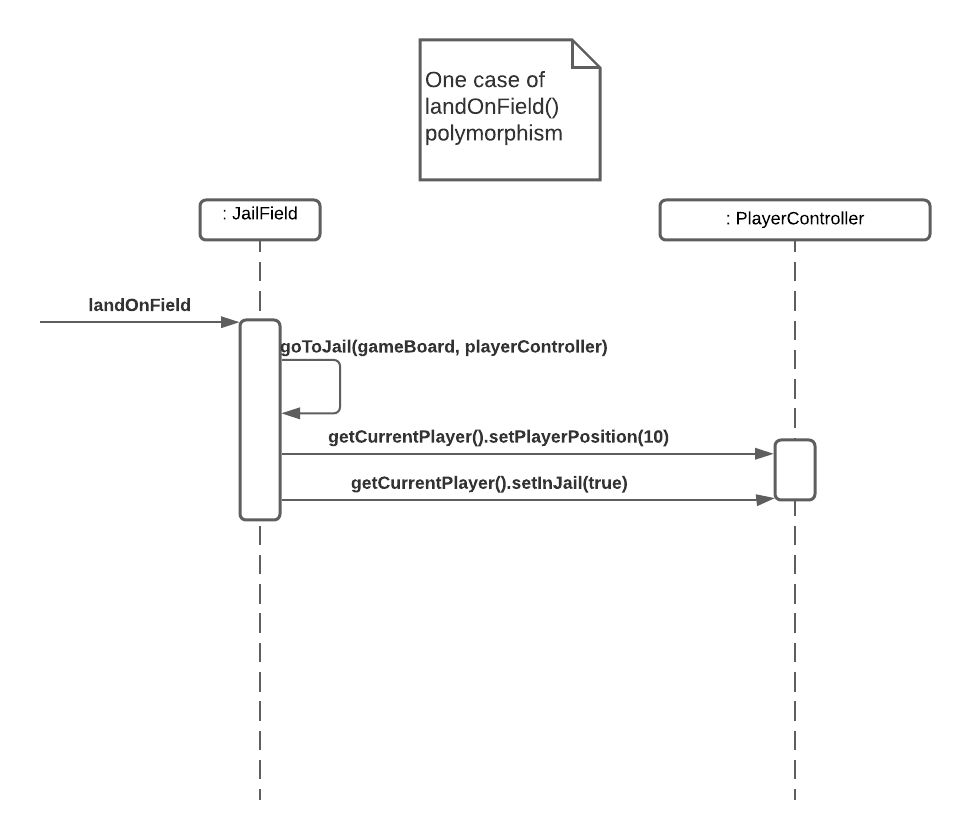
\includegraphics[width=13cm]{Report/figures/landOnField_sekvens.png}
    \caption{Sekvensdiagram over landOnField polymorphism.}
    \label{landOnField}
\end{figure}

\subsection{Klassediagram}
Gameloop klassen danner nye objekter af klasserne Menu, Jail, Language, Rules, DieController, GameBoard, GUIController og PlayerController (se Figure \ref{Klassediagram}) - for en oversigt af de forskellige klasser se Figure \ref{Klasse_chancekort} til \ref{Klasse_GUIController}. Herefter køres størstedelen af spillogikken i Gameloop klassen, hvor hver controller har sin egen logik.
\addlinespace[0.5cm]


\begin{figure}[H]
    \centering
    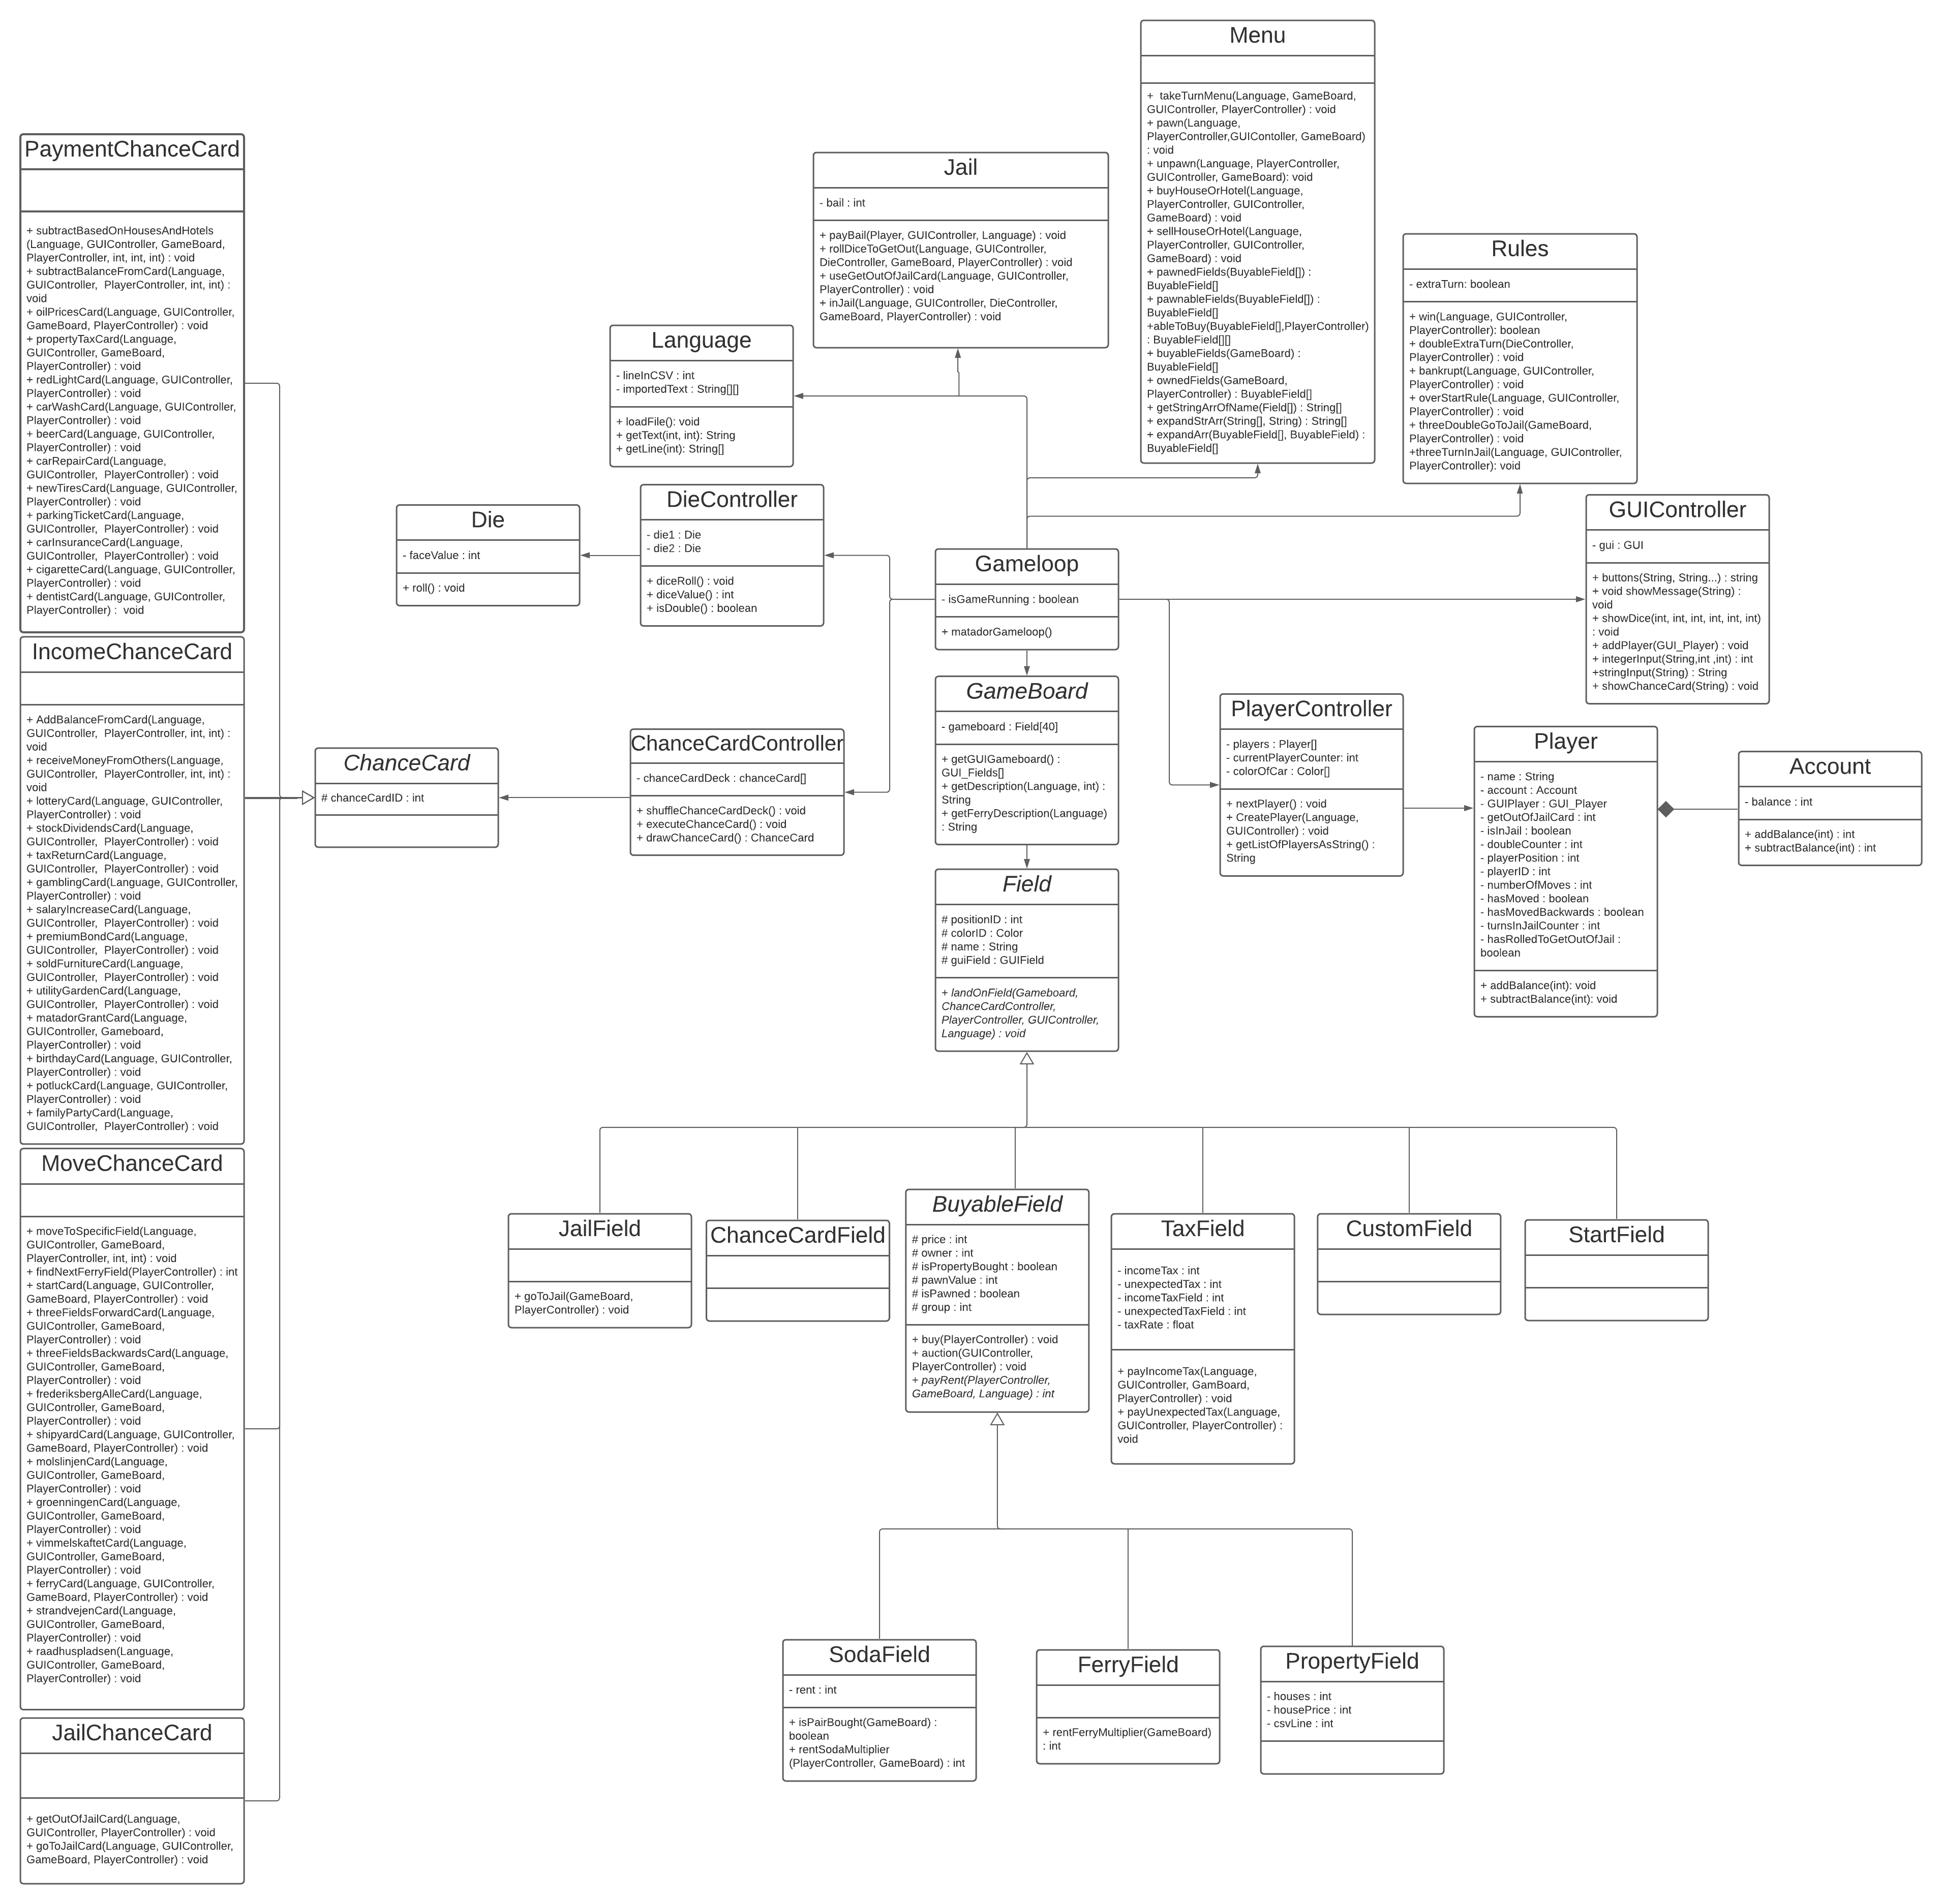
\includegraphics[width=16cm, height = 20cm]{Report/figures/Klassediagram/klassediagram_storenavne.png}
    \caption{Overordnet klassediagram}
    \label{Klassediagram}
\end{figure}

\begin{figure}[H]
    \centering
    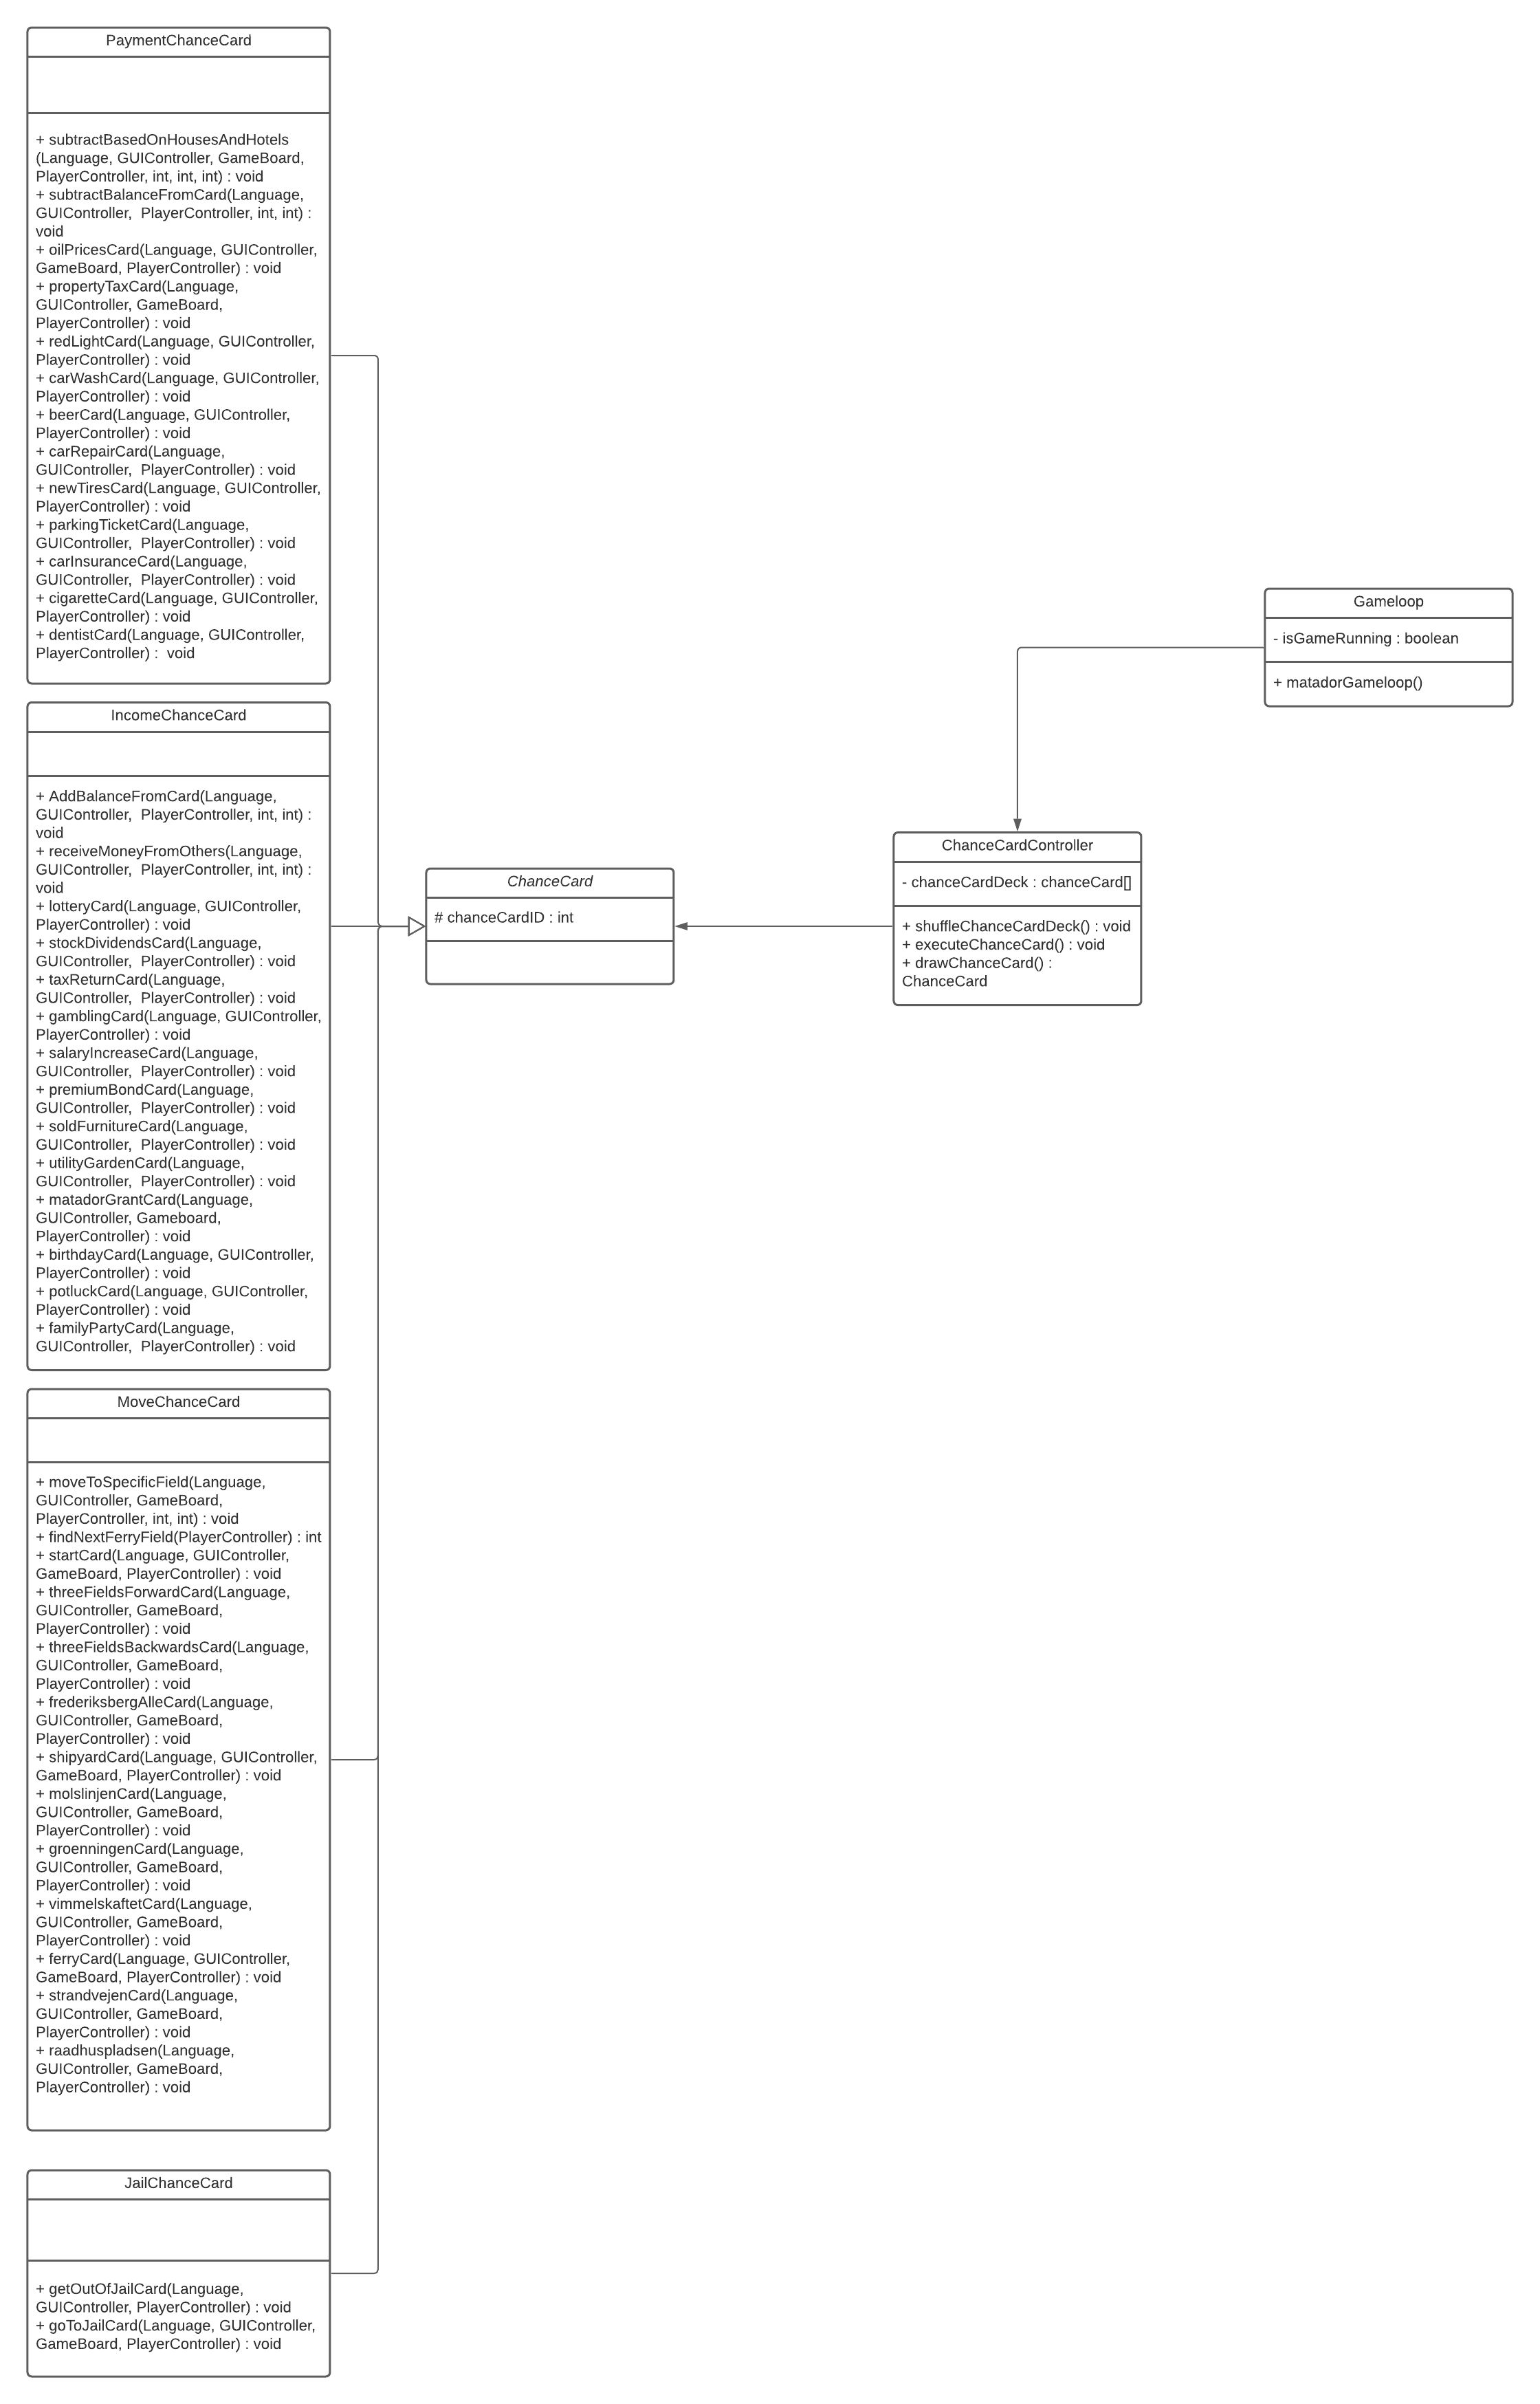
\includegraphics[width=14cm]{Report/figures/Klassediagram/ChanceCard_klassediagram.png}
    \caption{Klassediagram over chancekort.}
    \label{Klasse_chancekort}
\end{figure}


\begin{figure}[H]
    \centering
    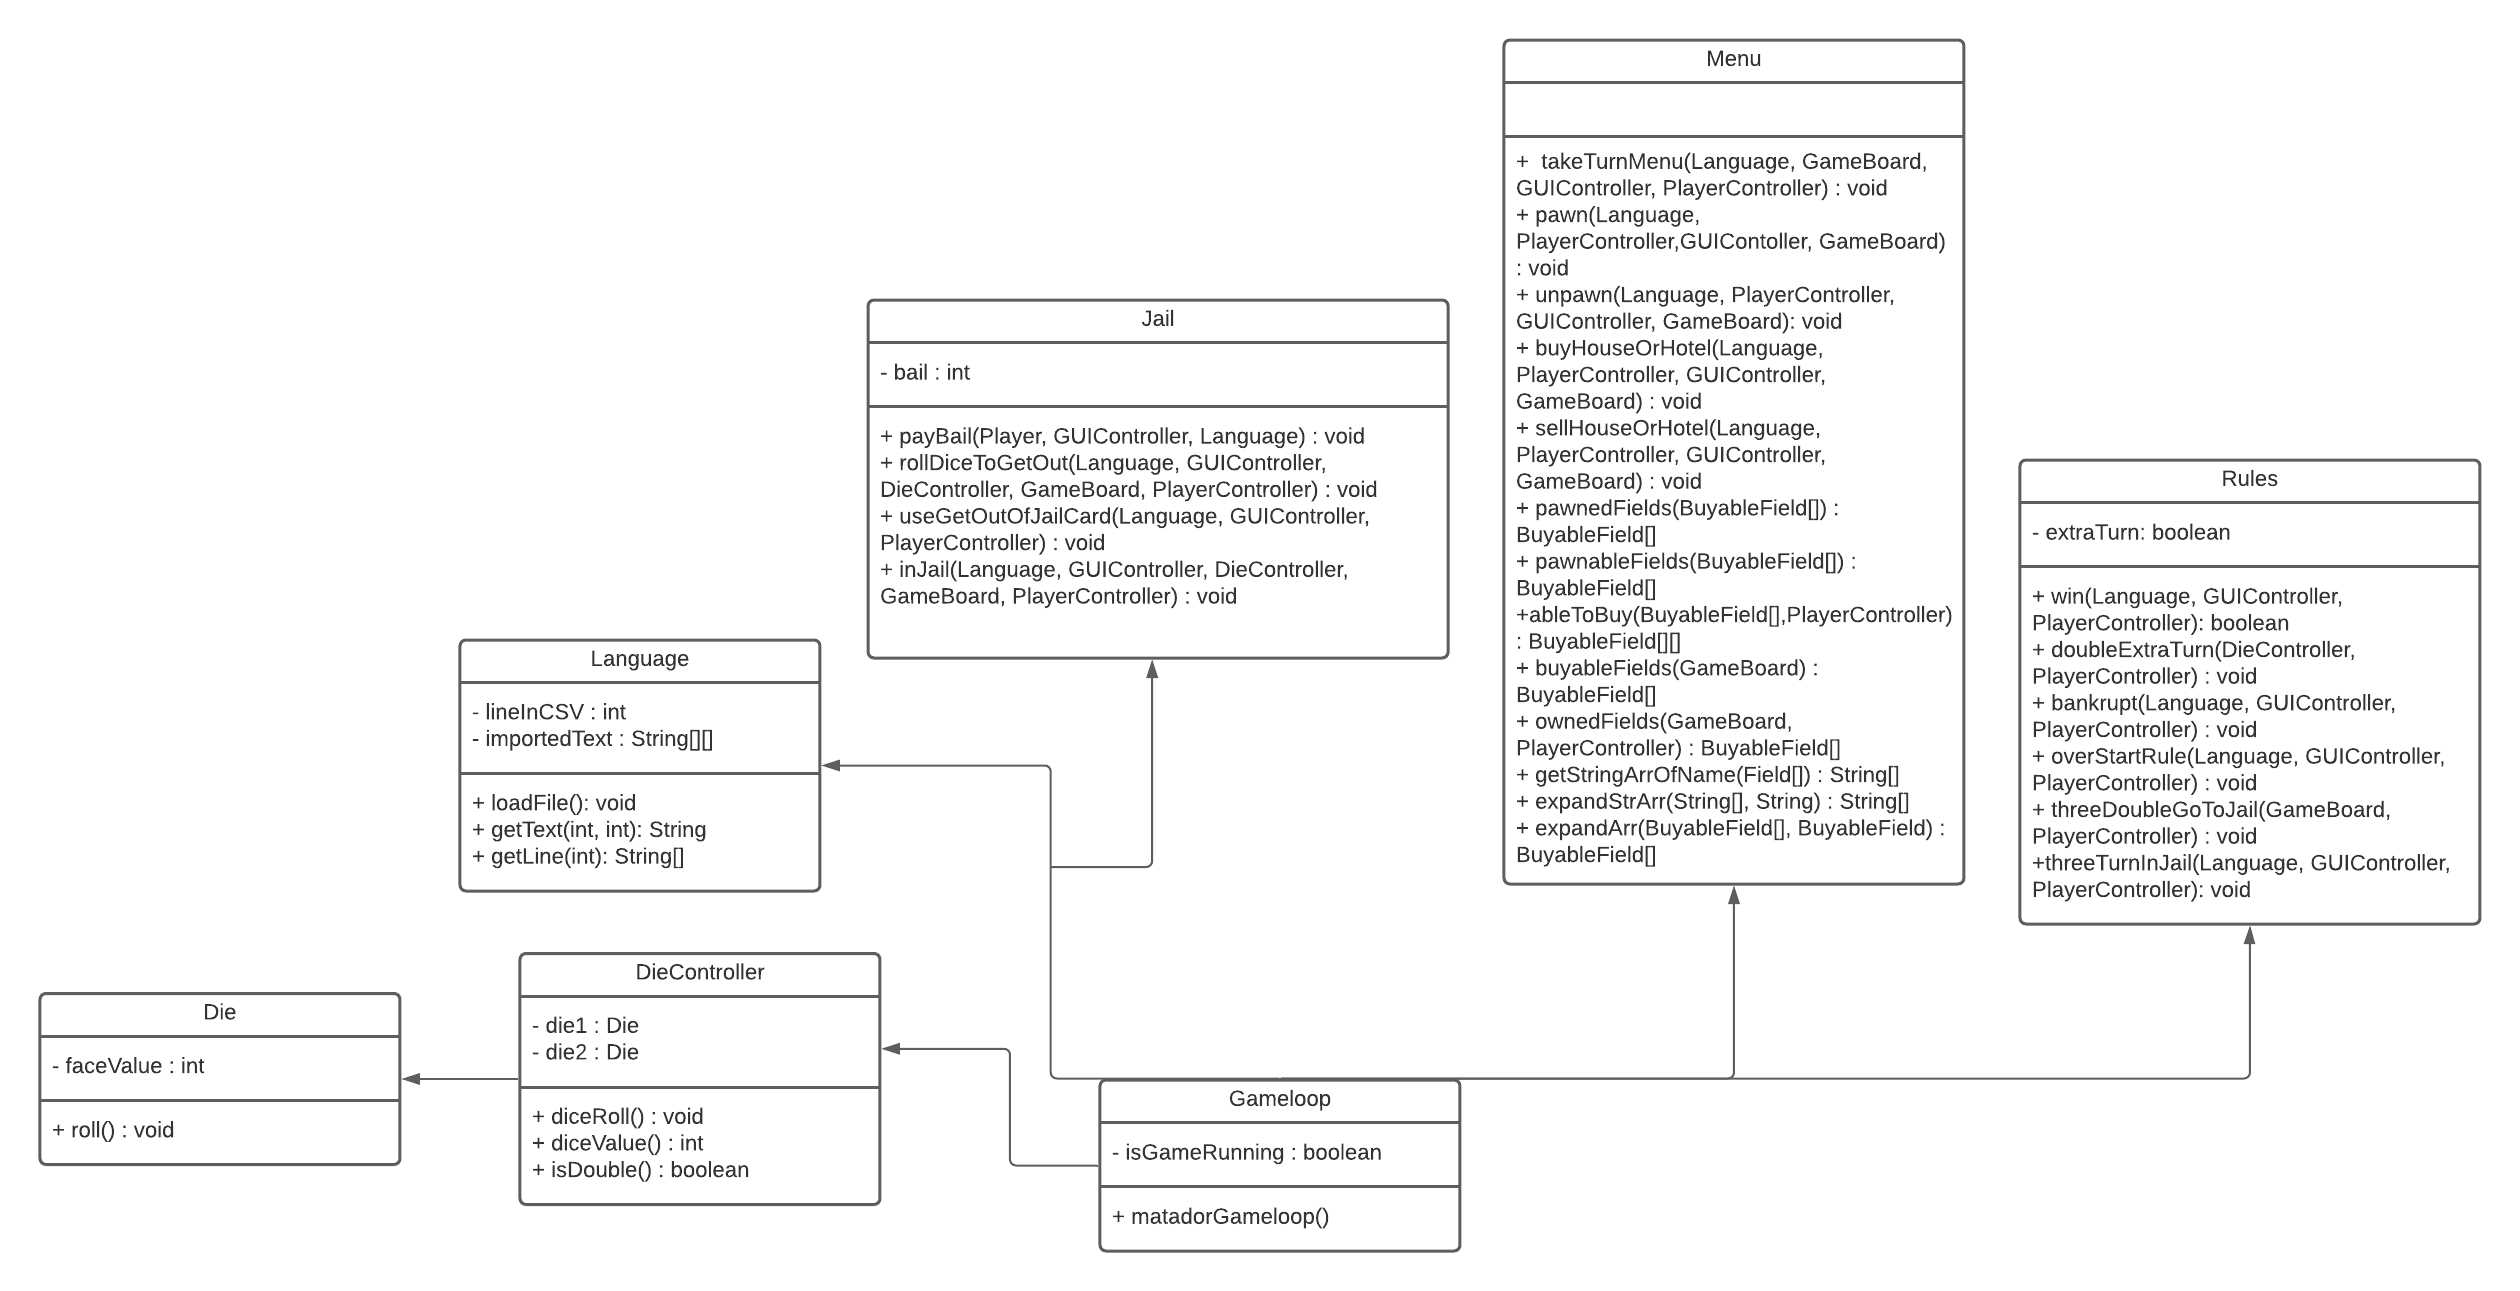
\includegraphics[width=15cm]{Report/figures/Klassediagram/DieController_Language_Jail_Men_Rule_klassediagram.png}
    \caption{Klassediagram over Language, DieController, Language, Jail, Menu og Rules.}
    \label{Klasse_Menu}
\end{figure}\begin{figure}[H]
    \centering
    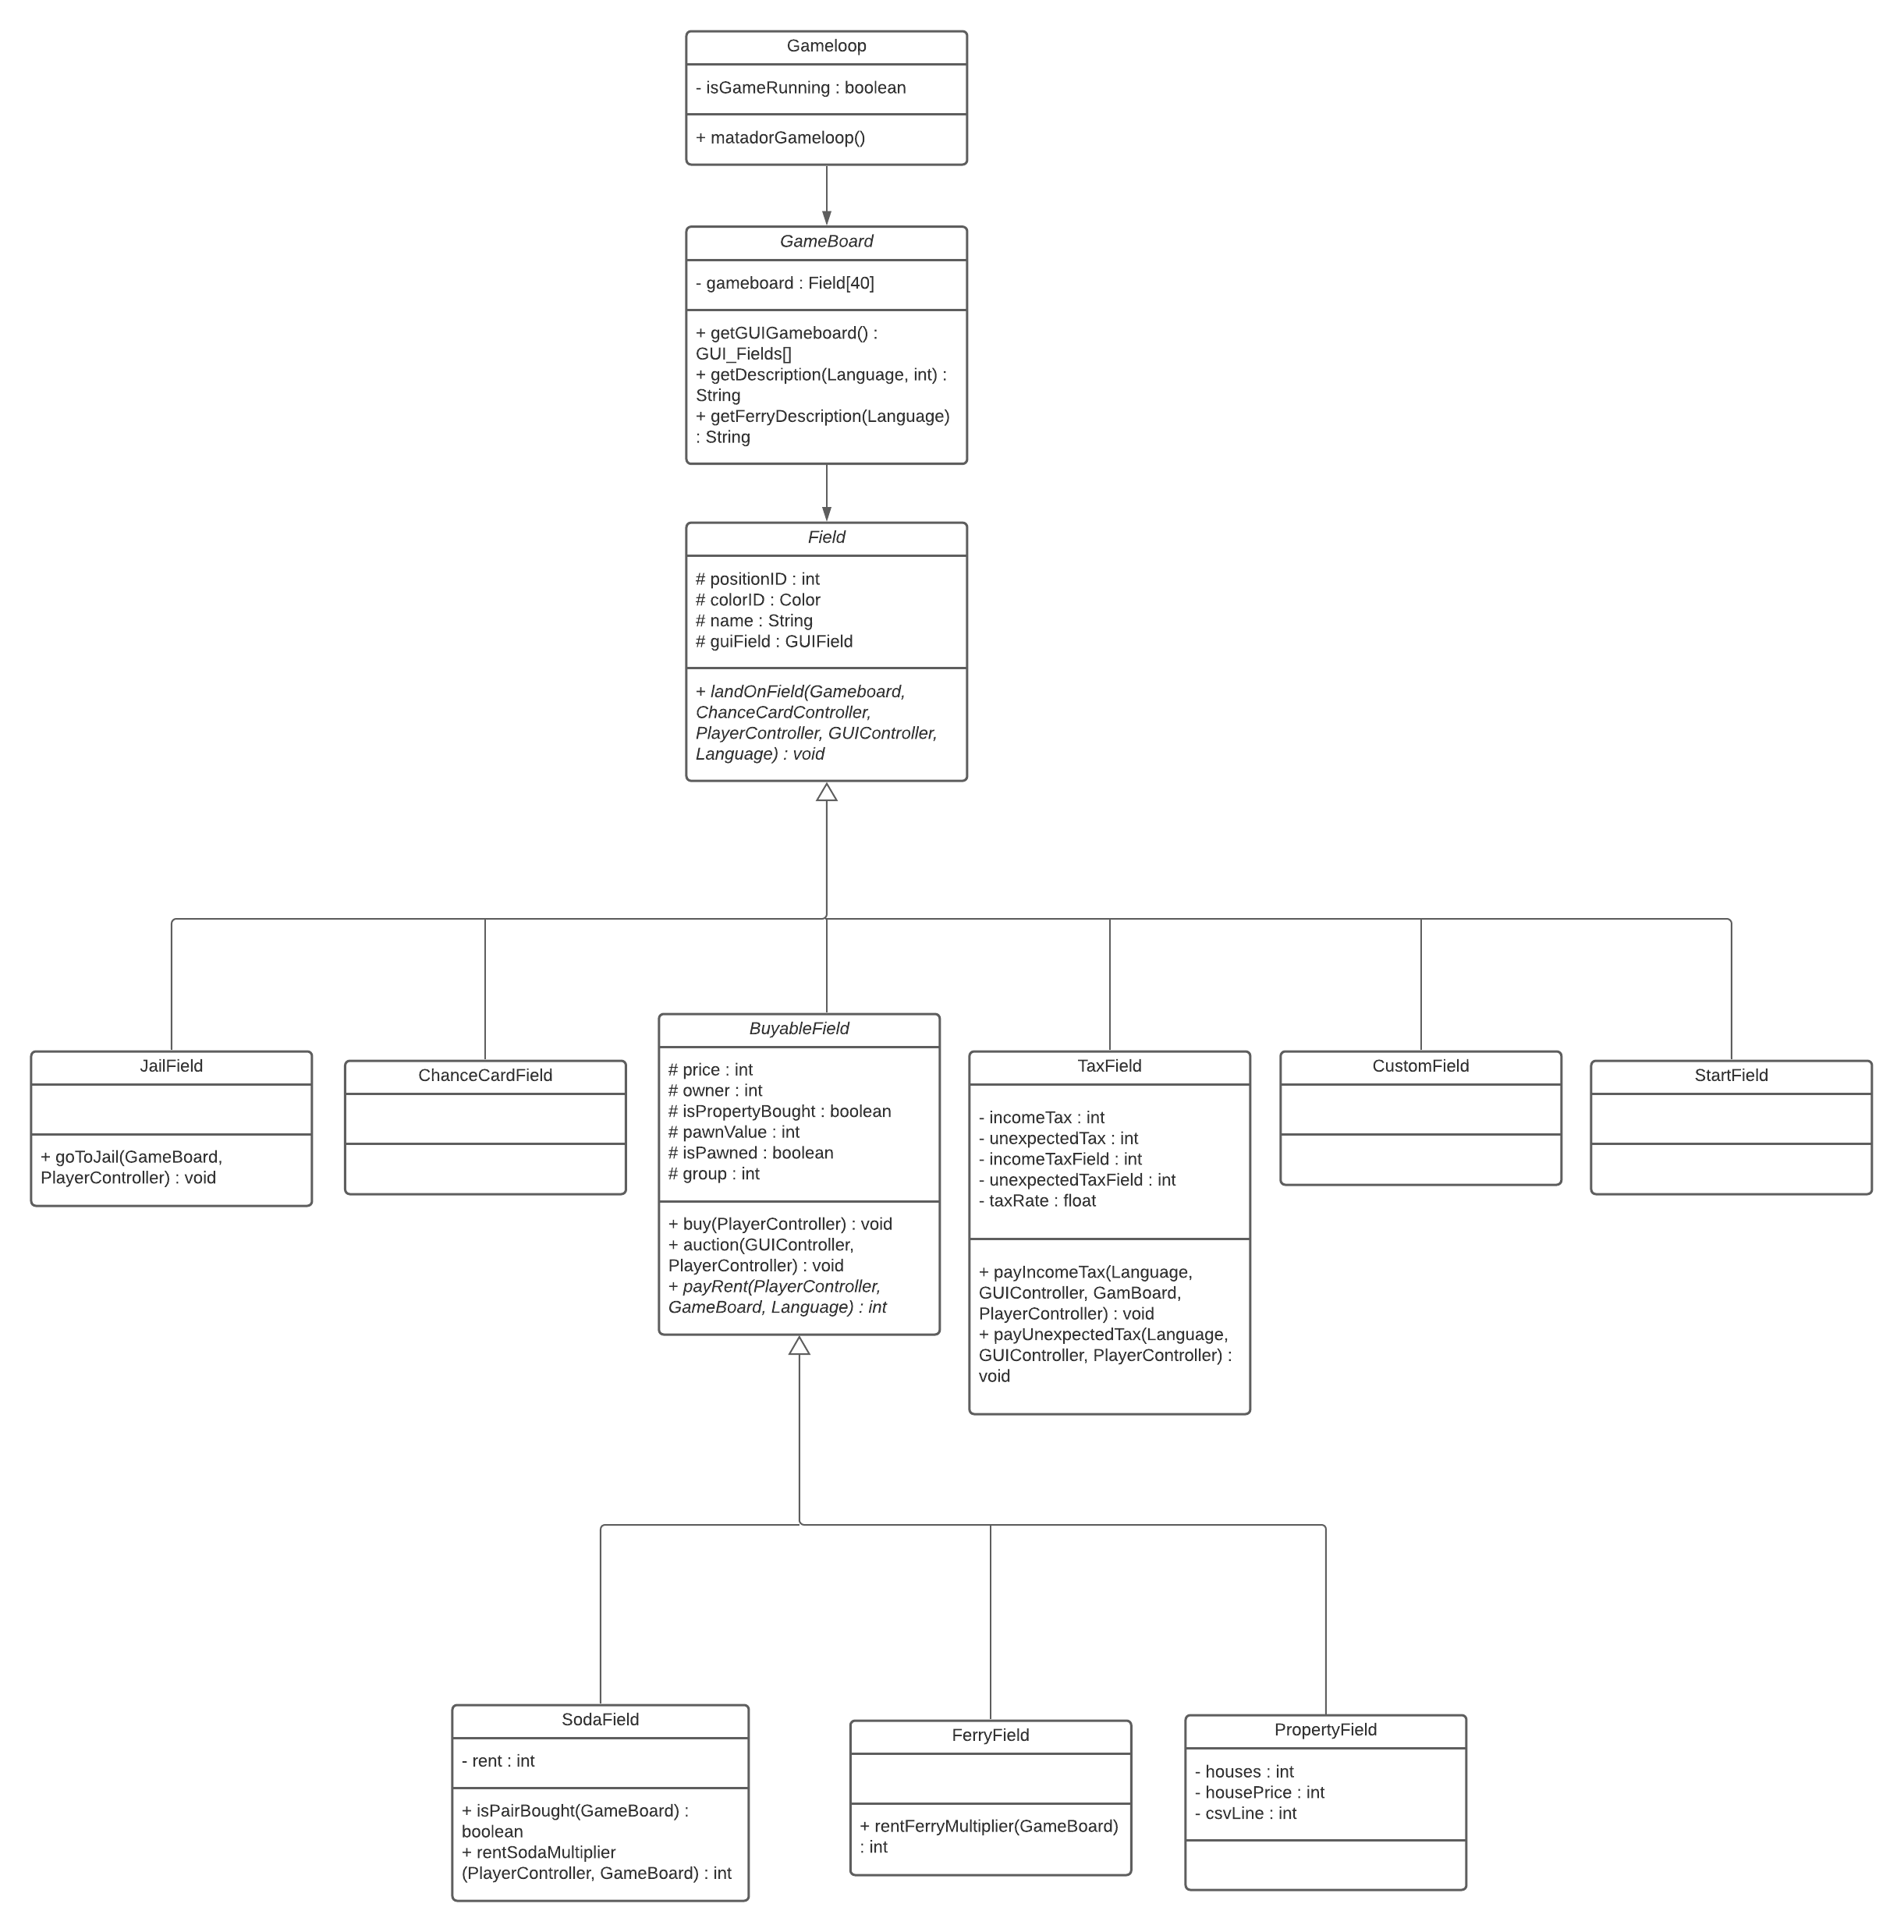
\includegraphics[width=15cm]{Report/figures/Klassediagram/Field_klassediagram.png}
    \caption{Klassediagram over Field klasser.}
    \label{Klasse_Field}
\end{figure}\begin{figure}[H]
    \centering
    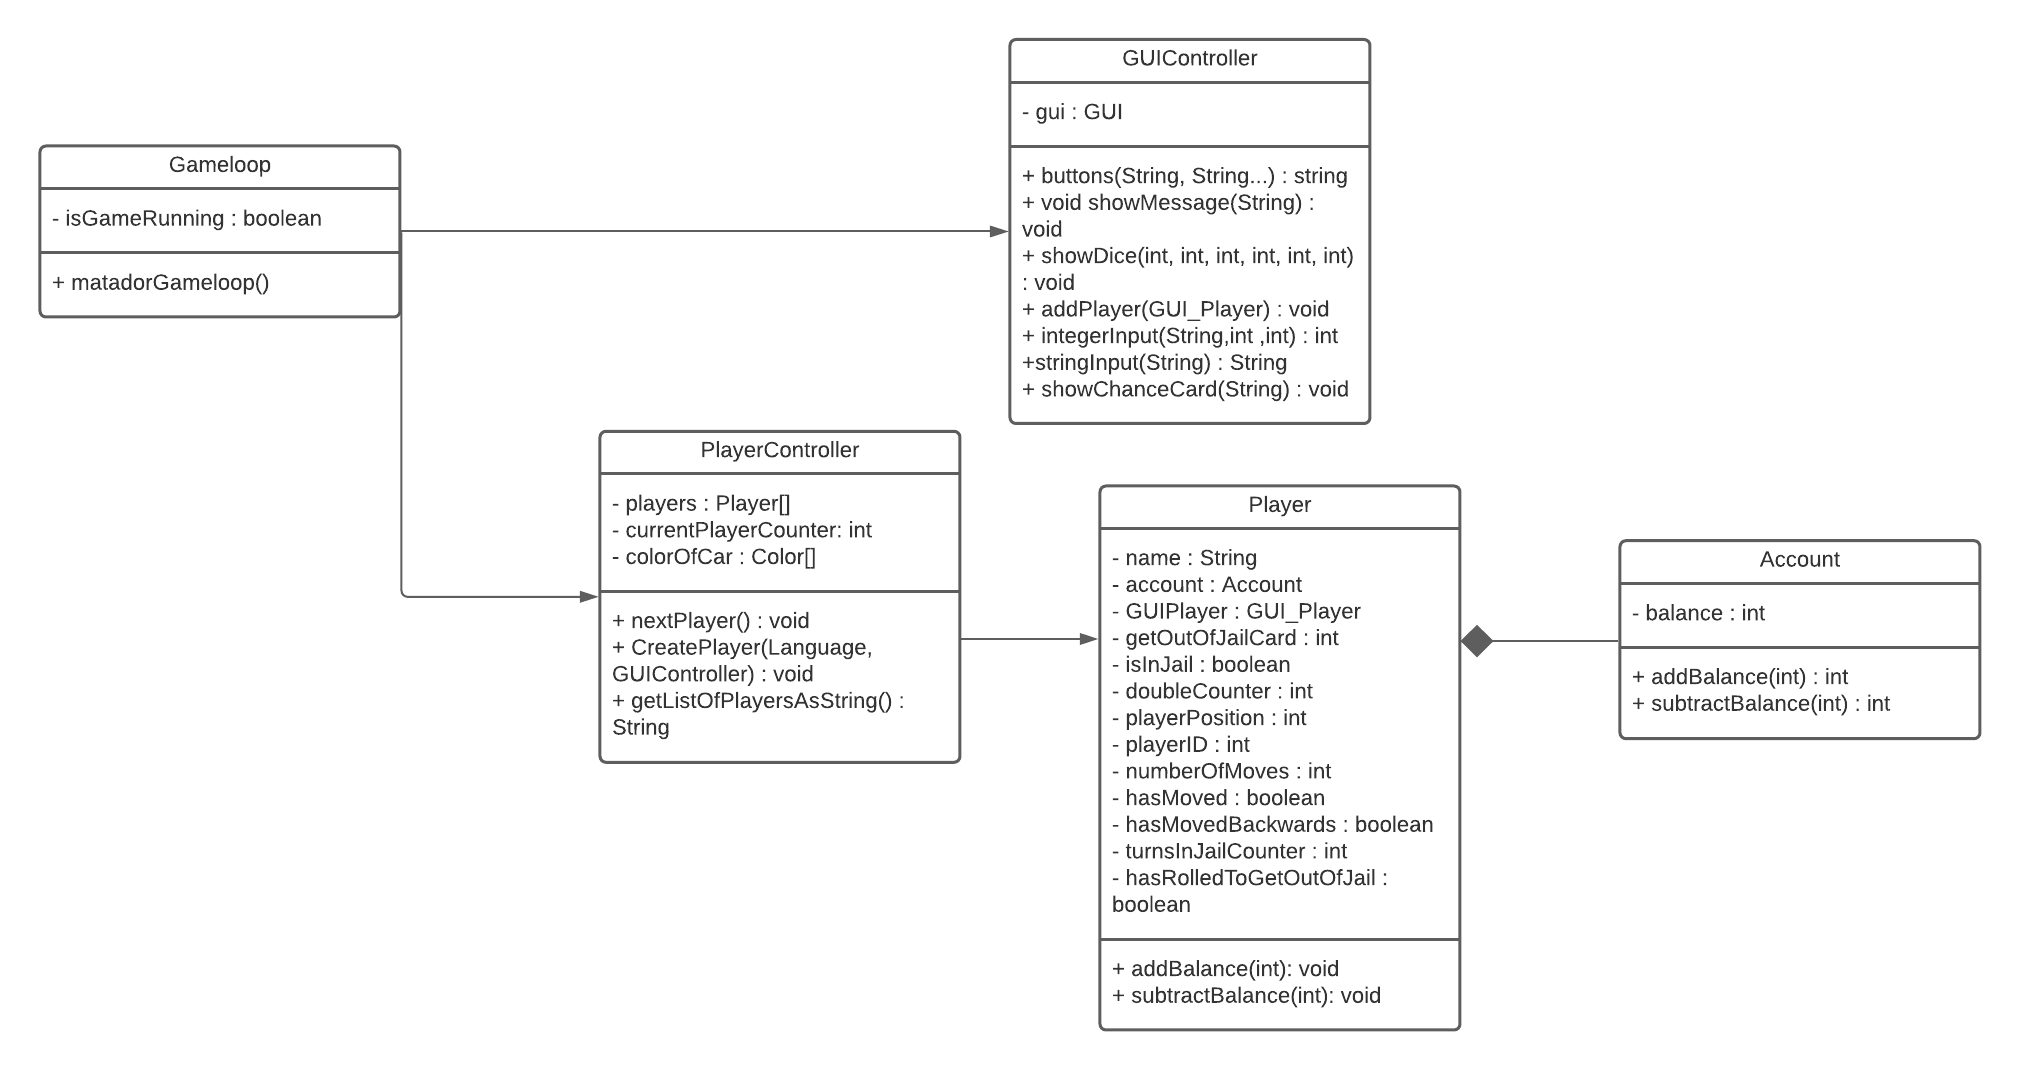
\includegraphics[width=15cm]{Report/figures/Klassediagram/player_GUIController_klassediagram.png}
    \caption{Klassediagram over GUIcontroller.}
    \label{Klasse_GUIController}
\end{figure}


\end{flushleft}